\documentclass{article}


\usepackage{PRIMEarxiv}

\usepackage[utf8]{inputenc} % allow utf-8 input
\usepackage[T1]{fontenc}    % use 8-bit T1 fonts
\usepackage{hyperref}       % hyperlinks
\usepackage{url}            % simple URL typesetting
\usepackage{booktabs}       % professional-quality tables
\usepackage{amsfonts}       % blackboard math symbols
\usepackage{nicefrac}       % compact symbols for 1/2, etc.
\usepackage{microtype}      % microtypography
\usepackage{lipsum}
\usepackage{fancyhdr}       % header
\usepackage{graphicx}       % graphics
\graphicspath{{media/}}     % organize your images and other figures under media/ folder

\usepackage{amsmath}
\usepackage{lscape}

%Header
\pagestyle{fancy}
\thispagestyle{empty}
\rhead{ \textit{ }} 

% Update your Headers here
\fancyhead[LO]{Next-Concept Prediction}
% \fancyhead[RE]{Firstauthor and Secondauthor} % Firstauthor et al. if more than 2 - must use \documentclass[twoside]{article}



  
%% Title
\title{Next-Concept Prediction / Gamma-Neighborhood Model
%%%% Cite as
%%%% Update your official citation here when published 
\thanks{\textit{\underline{Citation}}: 
\textbf{Authors. Title. Pages.... DOI:000000/11111.}} 
}

\author{
  Evin Tunador \\
  Independent \\
  \texttt{evintunador@gmail.com} \\
  %% examples of more authors
   \And
  Sammy Fellah \\
  Virginia Tech \\
  Blacksburg, VA\\
  \texttt{email@email} \\
  %% \AND
  %% Coauthor \\
  %% Affiliation \\
  %% Address \\
  %% \texttt{email} \\
  %% \And
  %% Coauthor \\
  %% Affiliation \\
  %% Address \\
  %% \texttt{email} \\
  %% \And
  %% Coauthor \\
  %% Affiliation \\
  %% Address \\
  %% \texttt{email} \\
}


\begin{document}
\maketitle


\begin{abstract}
\end{abstract}


% keywords can be removed
\keywords{Token \and Concept \and More}


\section{Introduction}

So to see the math take a look at figures \ref{fig:ncp_i=1_inf} through \ref{fig:ncp_i>1_train} and then the accompanying \texttt{next-concept\_predictor\_v8.6\_walkthrough.ipynb} jupyter notebook. Section \ref{sec:inspo} describes my inspirations for building the architecture, Section \ref{sec:regular} describes how a regular GPT works so that you have something to compare my weird formatting and figures to, and Section \ref{sec:NCP} walks you through inference with my next-concept predictor algorithm.

\section{Inspiration}
\label{sec:inspo}

For a detailed and more lively walkthrough of these inspiration explanations, check out \hyperlink{https://youtu.be/Ipl4v_rp2_A}{this youtube video}.\par

\subsection{pause tokens and dynamic computational width}
One of our primary goals here is to give the models a chance to think a bit before they speak. 
The most recent example of researchers trying to do this can be found in \cite{goyal2023think}, but I think their implementation is far inferior to ours.
Their method involves completely random injection of "pause tokens" whereas ours allows the model to indicate when it needs more time to think, subject to hyperparameter $\gamma$.
Their addition of a single learnable pause token increases computational "width" (adding to the sequence length, aka widening the residual) which ours does as well.
However, our methodology involving dynamically created concept embedding vectors actually makes effective use of those extra tokens in the first residual stream rather than just adding a single static learnable token.
And finally, our method also allows for increased model "length" in the sense that the model gets to actually entirely run again and "retry" using these concept embedding vectors. \par

\subsection{transformers as operations in embedding space}
Another goal stems from \cite{singh2023analyzing} which lays out theory claiming that rather than thinking of transformers as holding information inside of all of their weights, we should think of all the information being stored in the embedding space, and the model layers as an operation that moves along the lowest-entropy path through embedding space.
Previously an embedding vector has always corresponded to the nearest token embedding vector. 
Here, if the model outputs an embedding vector that is not sufficiently close to a token, we'll consider that a "concept embedding vector" and let the model try again with the addition of this new concept embedding vector in its sequence.
This means the model gets to use some of its own output as input to try again, essentially allowing the model to "think" to itself.\par

\subsection{consciousness as an RL algorithm}
Our third and final goal stems from my own intuition about reinforcement learning and consciousness.
Reinforcement Learning people often scream about strict definitions for what counts as reinforcement learning (such as claims that RLHF doesn't count) which are fair in most contexts.
However, here allow me to generalize a bit.
I believe the levels of consciousness are a set of nested RL algorithms.
for a better explanation than what i'm about to give here, see \hyperlink{https://youtu.be/119r0w5TMo0}{this video of mine} 
\begin{enumerate}
    \item Take an agent acting in an environment; the simplest possible strategy is to learn actions that best minimize loss given states of the environment, essentially a Q-learning lookup table aka memorization.
    \item The better strategy is to construct an actual internal model\footnote{
        define an internal model as a minimal or near minimal dimensional representation that is isomorphic (if minimal) or approaches (if near minimal) the intrinsic dimensionality of the system
    } of the environment.
    Such an internal model, if correct, would allow for generalization to out-of-distribution data points because the model actually "understands"\footnote{
        on a side-note, i've actually got this sick af definitions of 1) understanding, 2) creativity and 3) consciousness in terms of their computational aspects that i'm working on with a buddy rn. it's so exciting i think i'm really onto something. see this video https://youtu.be/119r0w5TMo0
    } the relationship between the environment state and loss rather than having memorized environment states it has already seen in training. 
    Thanks to this "understanding" rather than memorizing, the model can generalize to o.o.d data (aka the test set).\footnote{
    see the grokking phenomenon for a good look at what i'm talking about in isolated synthetic environments.
    }
    \item In proper RL environments (i'm referring to markov decision processes), the agent's actions actually effect the environment's state in the future. 
    As such, an even better strategy than the previous would be to not only maintain an internal model of the environment, but also model how the agent's own actions affect the environment.
    This would allow the agent to choose actions that optimize loss better in the sense of higher accuracy but also to take into account how their actions affect future time periods.
    \item Furthermore, why not have the agent maintain an internal model of itself to better predict what actions it might take, and therefore based on that model be capable of adjusting its own meta-strategies? 
    This is consciosuness, and so were the lower levels in the sense that we're defining consciousness as this algorithms involving recursive levels of awareness, aka the realization of what is actually "in" your environment (you are!).
    This is a relatively simple walkthrough; the problem gets far more complex when you take into account other agents and their consciousness, at which point we get 9-12+ levels in humans as described in 
    \begin{itemize}
        \item https://www.youtube.com/watch?v=kse87ocS0Uo
        \item https://www.youtube.com/watch?v=AbPM8dMxcDE
    \end{itemize}
\end{enumerate}
But anyways it is my belief that using the model's own output as occasional inputs (concept embedding vectors) we are beginning the first steps towards encouraging consciousness.
In order to most optimally utilize these concept embedding vectors, the model will have to \textit{understand} that they are actually coming from itself. 

\section{Regular Next-token predictor GPT}
\label{sec:regular}

Rather than delve right into the model, i'm going to first lay out the math for a regular GPT.
I'm reviewing a regular GPT because I want to make sure that you clearly understand the diagram structure i've created.\par

First, let's walk through a regular GPT as shown in figure \ref{fig:regular} so that later figures make more sense. I recommend following along with the provided jupyter notebook while reading this. \par

\begin{enumerate}
    \item We start with sequence $S$ shape $(b,n)$ and embedding matrix $E$ shape $(v,d)$ where $b$ is the batch size, $n$ is the sequence length, $v$ is the token vocabulary size, and $d$ is the embedding dimension fo the model.
    Perform an index matchup lookup to create residual $X_0$ of size $(b,n,d)$.
    \item Run through all $l$ layers of the GPT as normal. 
    That's right, i'm not going to explain GPT layers here. 
    In our model we will not actually be editing the layers.
    Now we've got final residual state $X_f$ of shape $(b,n,d)$.
    \item Here is the first part where our model will later transition away from the regular GPT. Multiply $X_f$ by $E^T$ shape $(d,v)$ to get $Z$ shape $(b,n,v)$.
    \item Select the last row along dimension $n$ from $Z$ and define it as $Z'$ shape $(b,v)$.
\end{enumerate}

Now our directions split into training vs inference.


\begin{figure}[!htb]
    \centering
    \begin{tabular}{cc}
        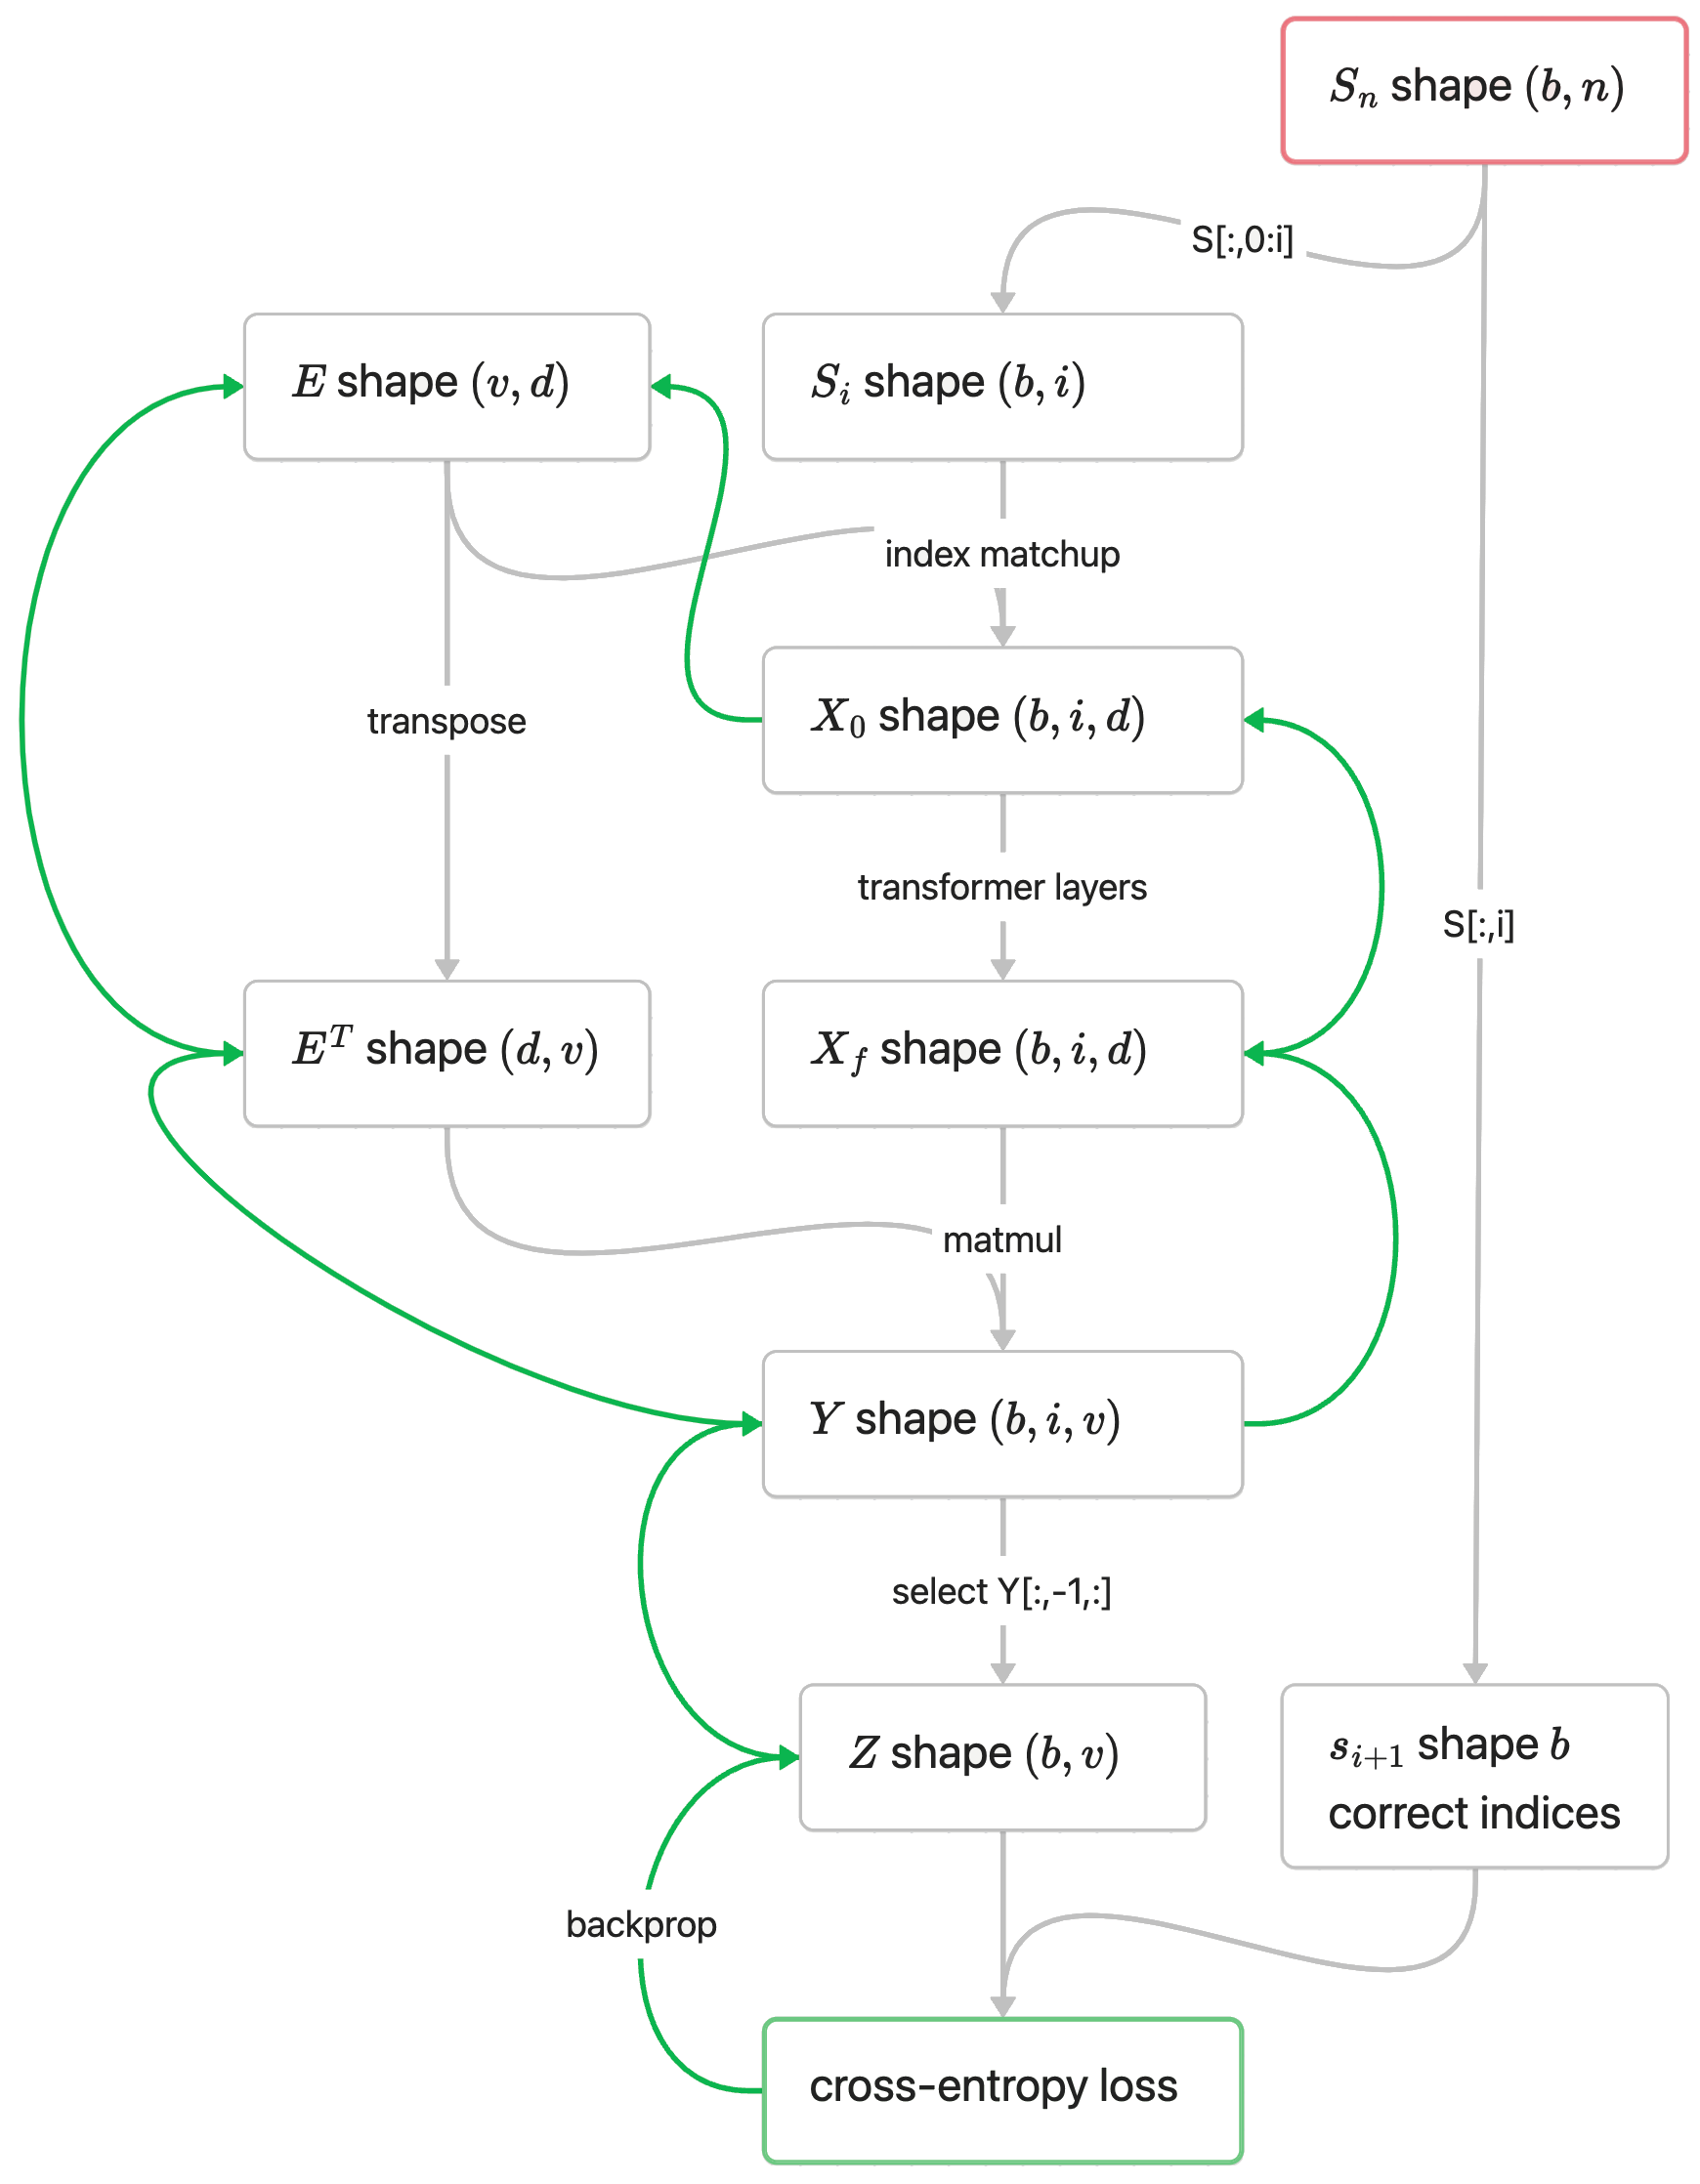
\includegraphics[width=0.45\textwidth]{NTP_train.png} & 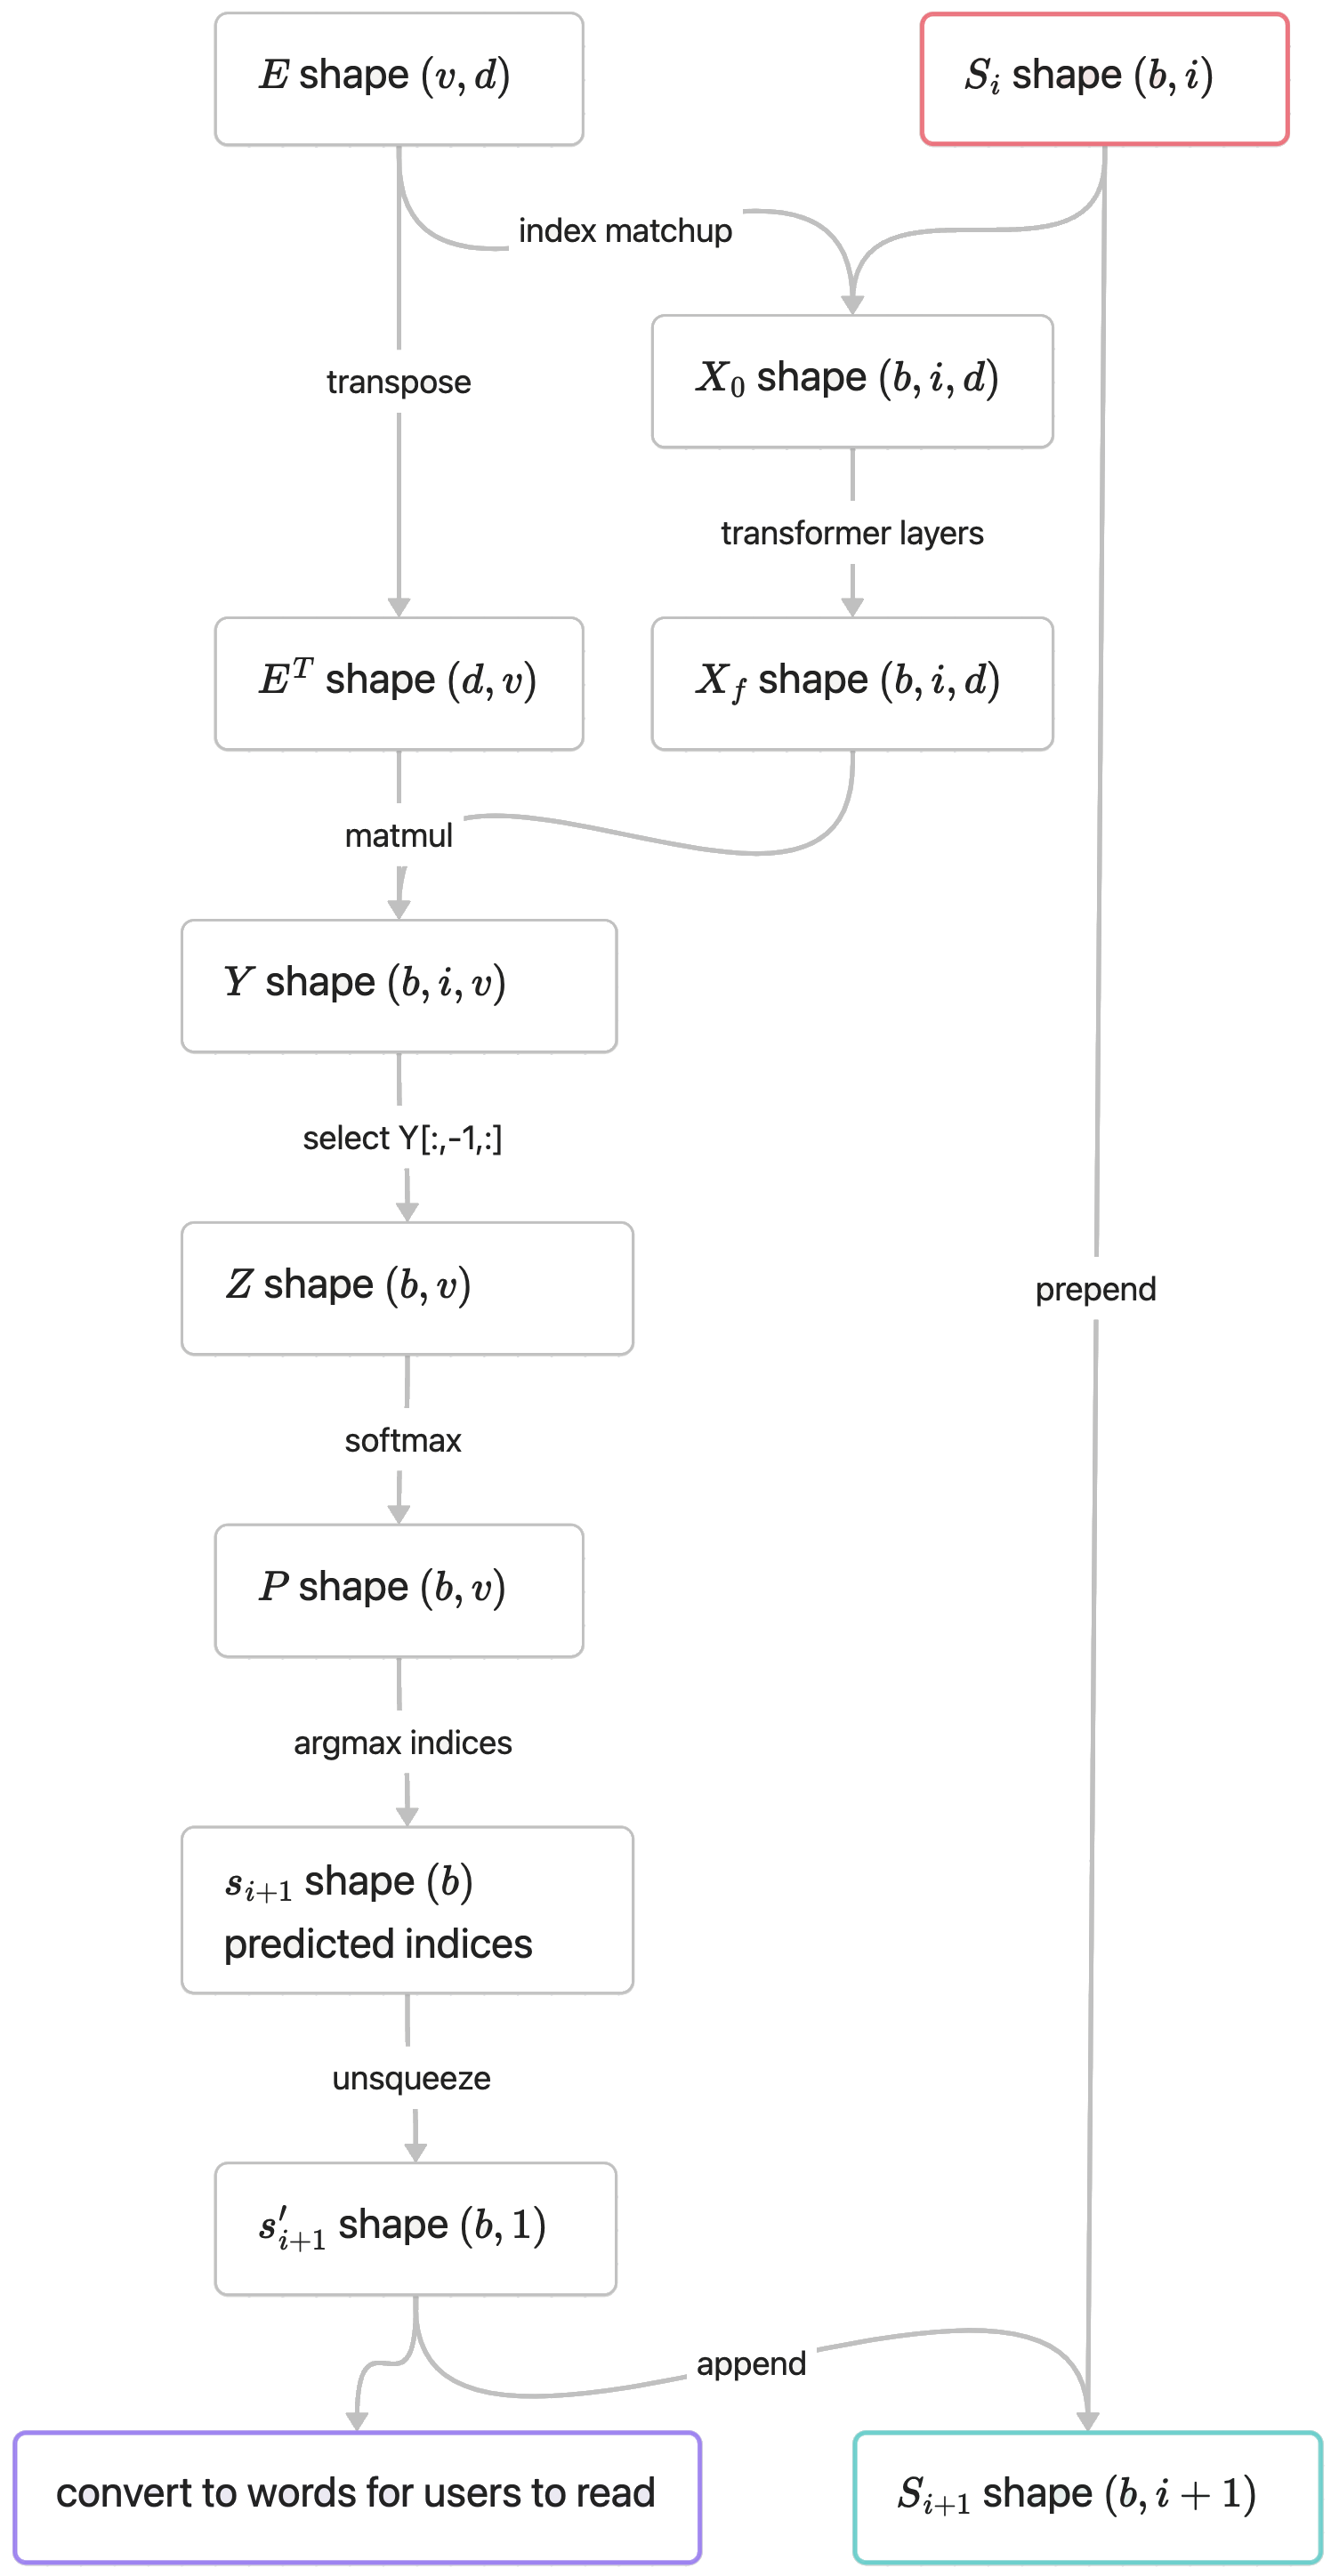
\includegraphics[width=0.45\textwidth]{NTP_inf.png} \\
        (a) & (b)
    \end{tabular}
    
    \caption{The way my diagram structure would work for training (a) and inference (b) with a regular next-token prediction GPT. Notice that i completely skip over the transformer layers which in reality are the bulk of the beast. We're only interested in the ending mechanism. Red means the object comes from the previous run or from context or the training set, purple means outputted to the user, blue means the object gets sent to be used during the next run, and green means used for backpropogation.}
    \label{fig:enter-label}
\end{figure}

\subsubsection{Training}
Define $S_{i+1}$ length $b$ as the list of correct indices for the tokens to be trained on. Perform cross-entropy loss between $S_{i+1}$ and $Z'$ and backprop the loss throughout the model.

\subsubsection{Inference}
\begin{enumerate}
    \item Perform a softmax along the $v$ dimension for $Z'$ to get $P$ shape $(b,v)$.
    \item Either grab the maximum probability (greedy decoding) or use the probabilities to find the index of your next token.
    \item Append this next token (a tensor of length $b$ full of integer indices if you're performing inference in a parallel batch) to the sequence $S$ now shape $(b,n+1)$. 
    \item Display the new token to the user and re-run the GPT with the new $S$ for the next token
\end{enumerate}





\section{My Model: GammaGPT? RoundGPT? ConceptGPT? Next-Concept Predictor? Next-Thought Predictor?}
\label{sec:NCP}

A key concept to understand here is a weird quirk of high dimensional vectors.
When we imagine what layernorm does, we think about it in 1, 2, or 3 dimensions at most.
At those dimensions, it looks like clumping points around the center at the origin and rarely points lie further out. 
However, in higher dimensions it turns out that layernorm actually effectively places vectors on the surface of a hyper-sphere.
As the number of entries in the vector ($d$) grows larger, the radius of this hyper-sphere also grows larger.
As $d$ increases the vectors actually maintain the same rough distance from the surface of this hyper-sphere, but when you look at them relative to the size of the hyper-sphere, you'll see they're converging towards its surface. 
Understanding of this is important because it's what allows us to use cosine similarity to judge the similarity between vectors even though cosine similarity ignores radius, thereby removing a degree of freedom and losing information.
In reality because these vectors are converging to the surface of the same hypersphere, they're already of dimensionality $d-1$ so no information is actually lost!
See figure \ref{fig:vectors} for a look at what this \textit{would} look like in 3 dimensions if it applied in 3 dimensions, and a comparison against how we usually visualize the effect of LayerNorm on vectors.\par

\begin{figure}[!htb]
    \centering
    \begin{tabular}{cc}
       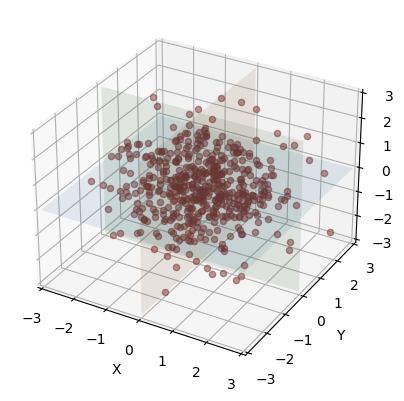
\includegraphics[width=0.4\textwidth]{layernorm_vectors.png}  &  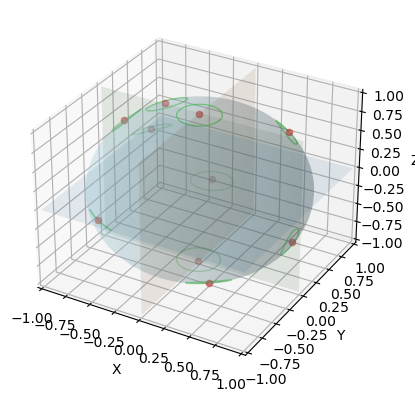
\includegraphics[width=0.4\textwidth]{gamma-neighborhoods.png}
    \end{tabular}
    
    \caption{Left: how we usually imagine the effect of LayerNorm on vectors, in this case with $d=3$ (more were shown for sake of clarity). 
    Right: How LayerNorm actually affects vectors of high dimension $d\gg 3$ (fewer were shown for clarity.}
    \label{fig:vectors}
\end{figure}

We'll be taking advantage of this structure in our model.
In figure \ref{fig:vectors} you'll see there are also green circles around each of the vectors on the sphere.
We'll call these $\gamma-$neighborhoods and make a small tweak to the output layer of a regular GPT such that it outputs an embedding vector length $d$ before creating the final classification logits.
If the embedding vector outputted by the model is within range of one of these $\gamma-$neighborhoods, it will be matched to a token as usual.
If the embedding vector outputted by the model is not within the range of one of these $\gamma-$neighborhoods, it will not be matched to a token and instead labeled as a concept vector $c$.
Concept vectors are appended to the sequence, and the model is run again. 
The value of hyperparameter $\gamma$ changes over the course of the sequence, essentially making the green circles wider and thus ensuring that the model does not get stuck outputting concept vectors in an infinite loop.
The green circles progressively get wider until there's no way to possibly be outside of them.\par

$0\leq\gamma<1$ is defined as a probability in reference to the post-softmax'ed model output.
If the token with highest probability $>\gamma$ then the model outputs that token, but if not then the model outputs the concept embedding vector that went into that softmax.
This probability threshold lowers for that individual sequence in the batch each time a concept vector is created.
Also, over the course of training epochs, the value that $\gamma$ starts at in the beginning of a sequence goes up.
Notice that $\gamma=0$ is equivalent to regular next-token prediction.
This means that at the beginning of pretraining our model will behave exactly like a regular next-token predictor.
It's only after $\gamma$ has grown to a high enough probability threshold that it starts defining the model's output as occasionally "not confident enough" and creating concept embedding vectors.\par

When you first look at figures \ref{fig:ncp_i=1_inf} through \ref{fig:ncp_i>1_train} they may seem intimidating compared to the earlier ones of a reagular next-token predictor. However, I hope if you walk through them and the accompanying jupyter notebook step-by-step you'll find that it's surprisingly simple. Really just a system of conditionals to select when we use a token vs a concept vector and when to train or output actual text. 

\begin{figure}[!htb]
    \centering
    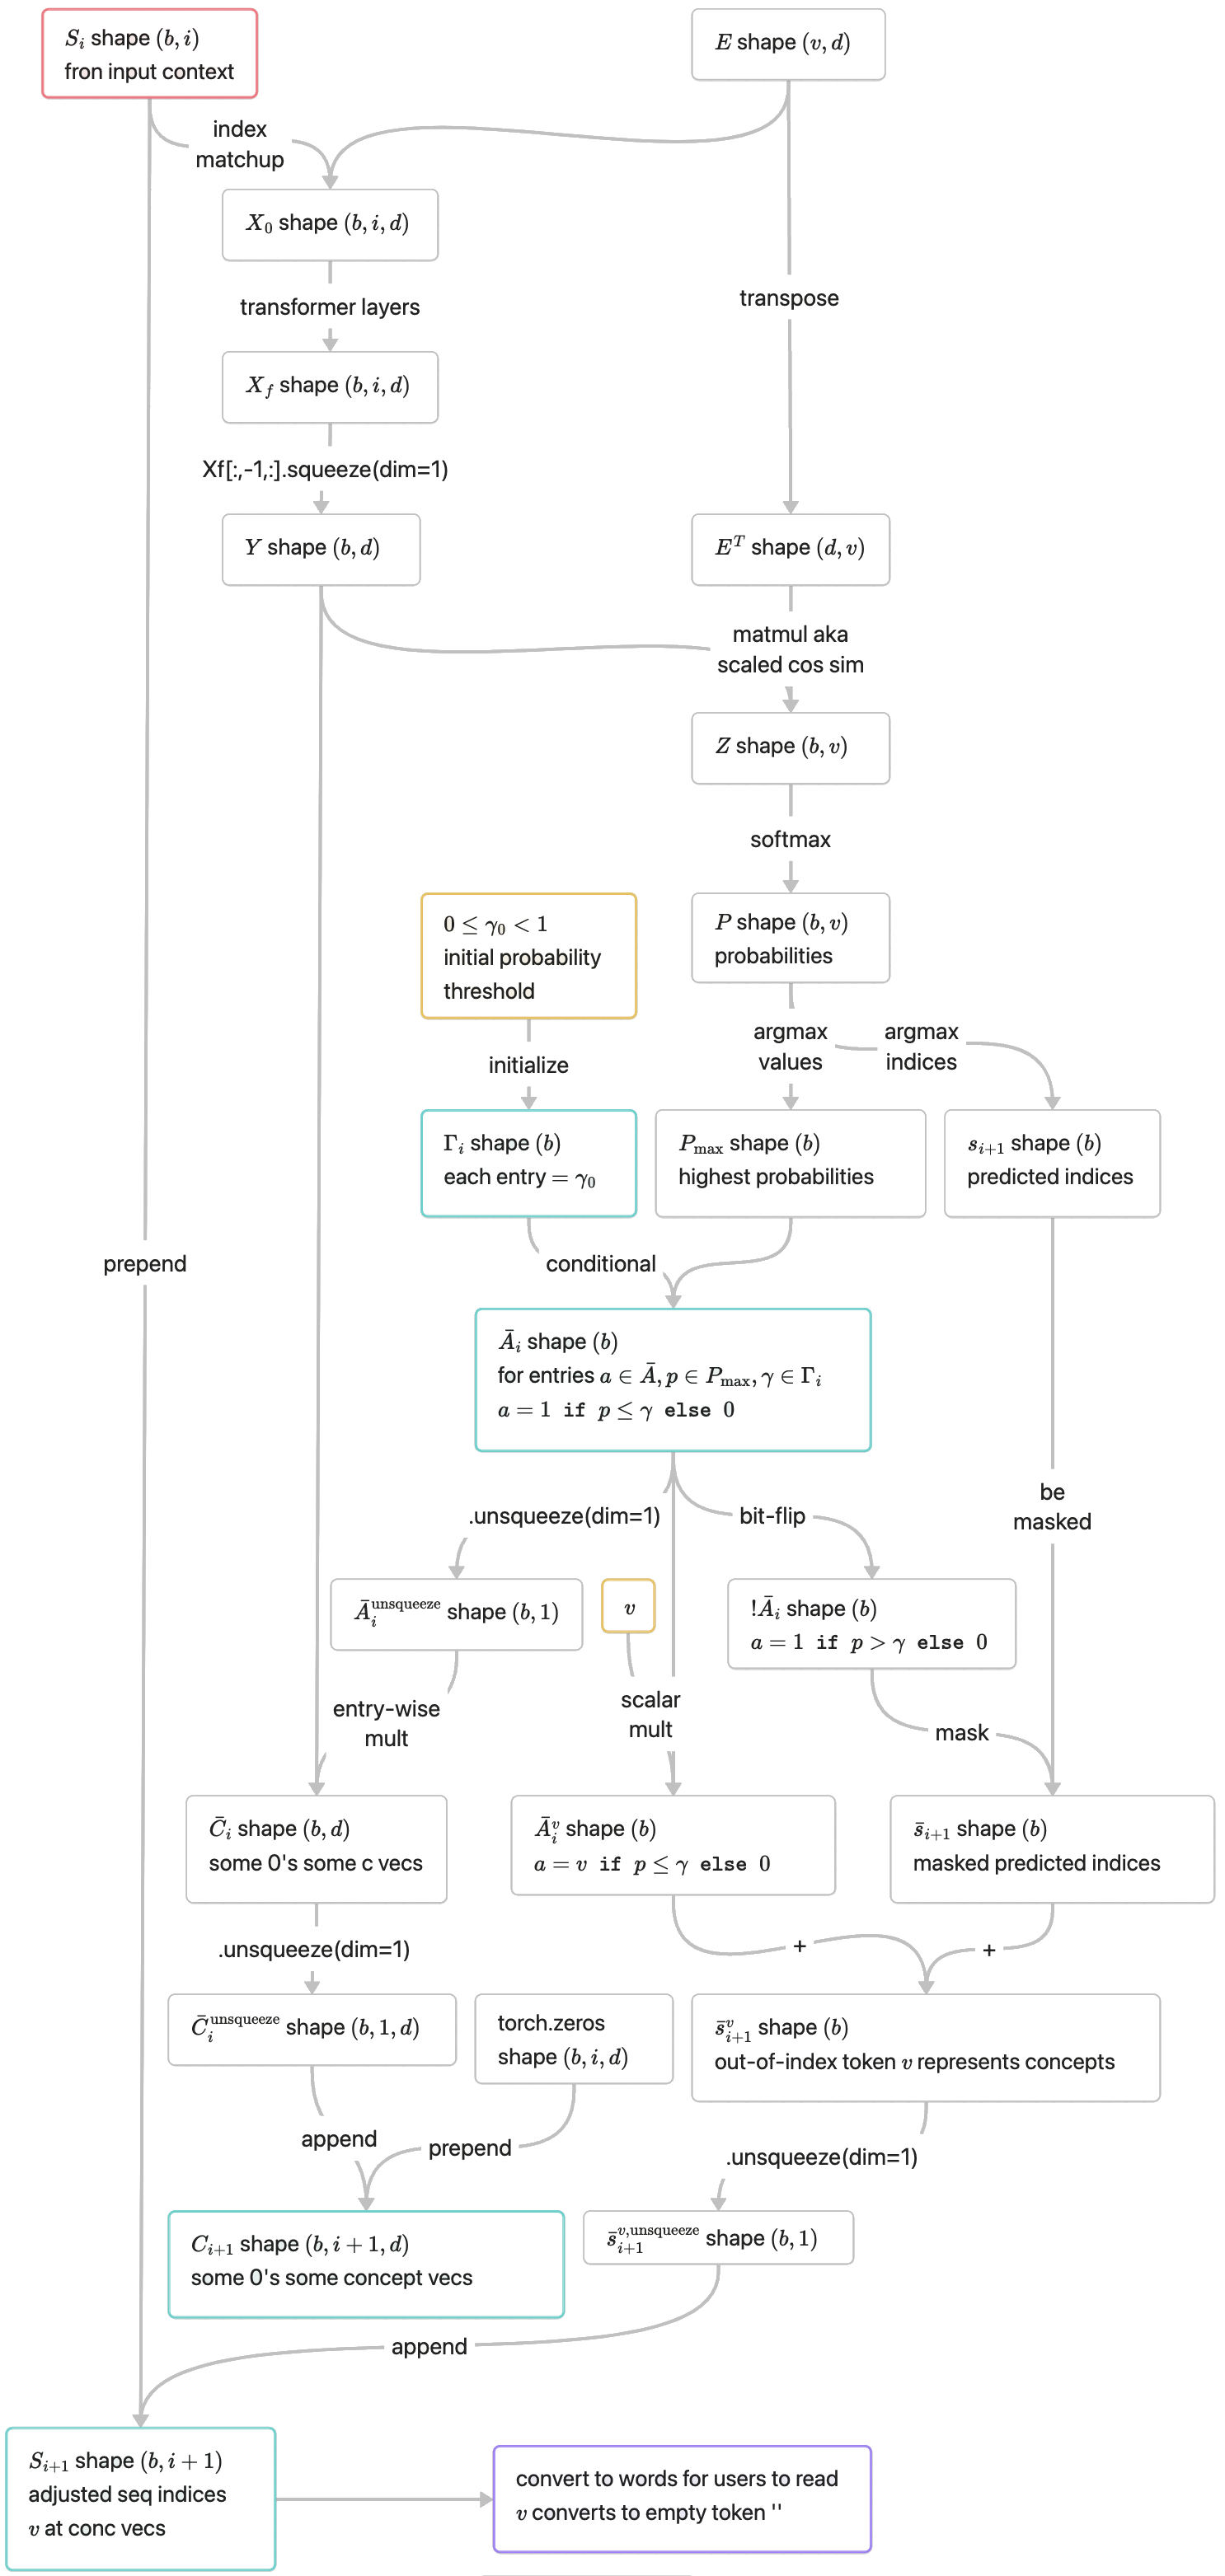
\includegraphics[height=0.86\textheight]{NCP_i=1_inf.png}
    \caption{The way my diagram structure would work for the first step $(i=1)$ of inference on my next-concept prediction GPT. A yellow box refers to a hyperparameter, red means the object comes from the previous run or from context or the training set, purple means outputted to the user, blue means the object gets sent to be used during the next run, and green means used for backpropogation.}
    \label{fig:ncp_i=1_inf}
\end{figure}

\newpage
\begin{figure}[!htb]
    \centering
    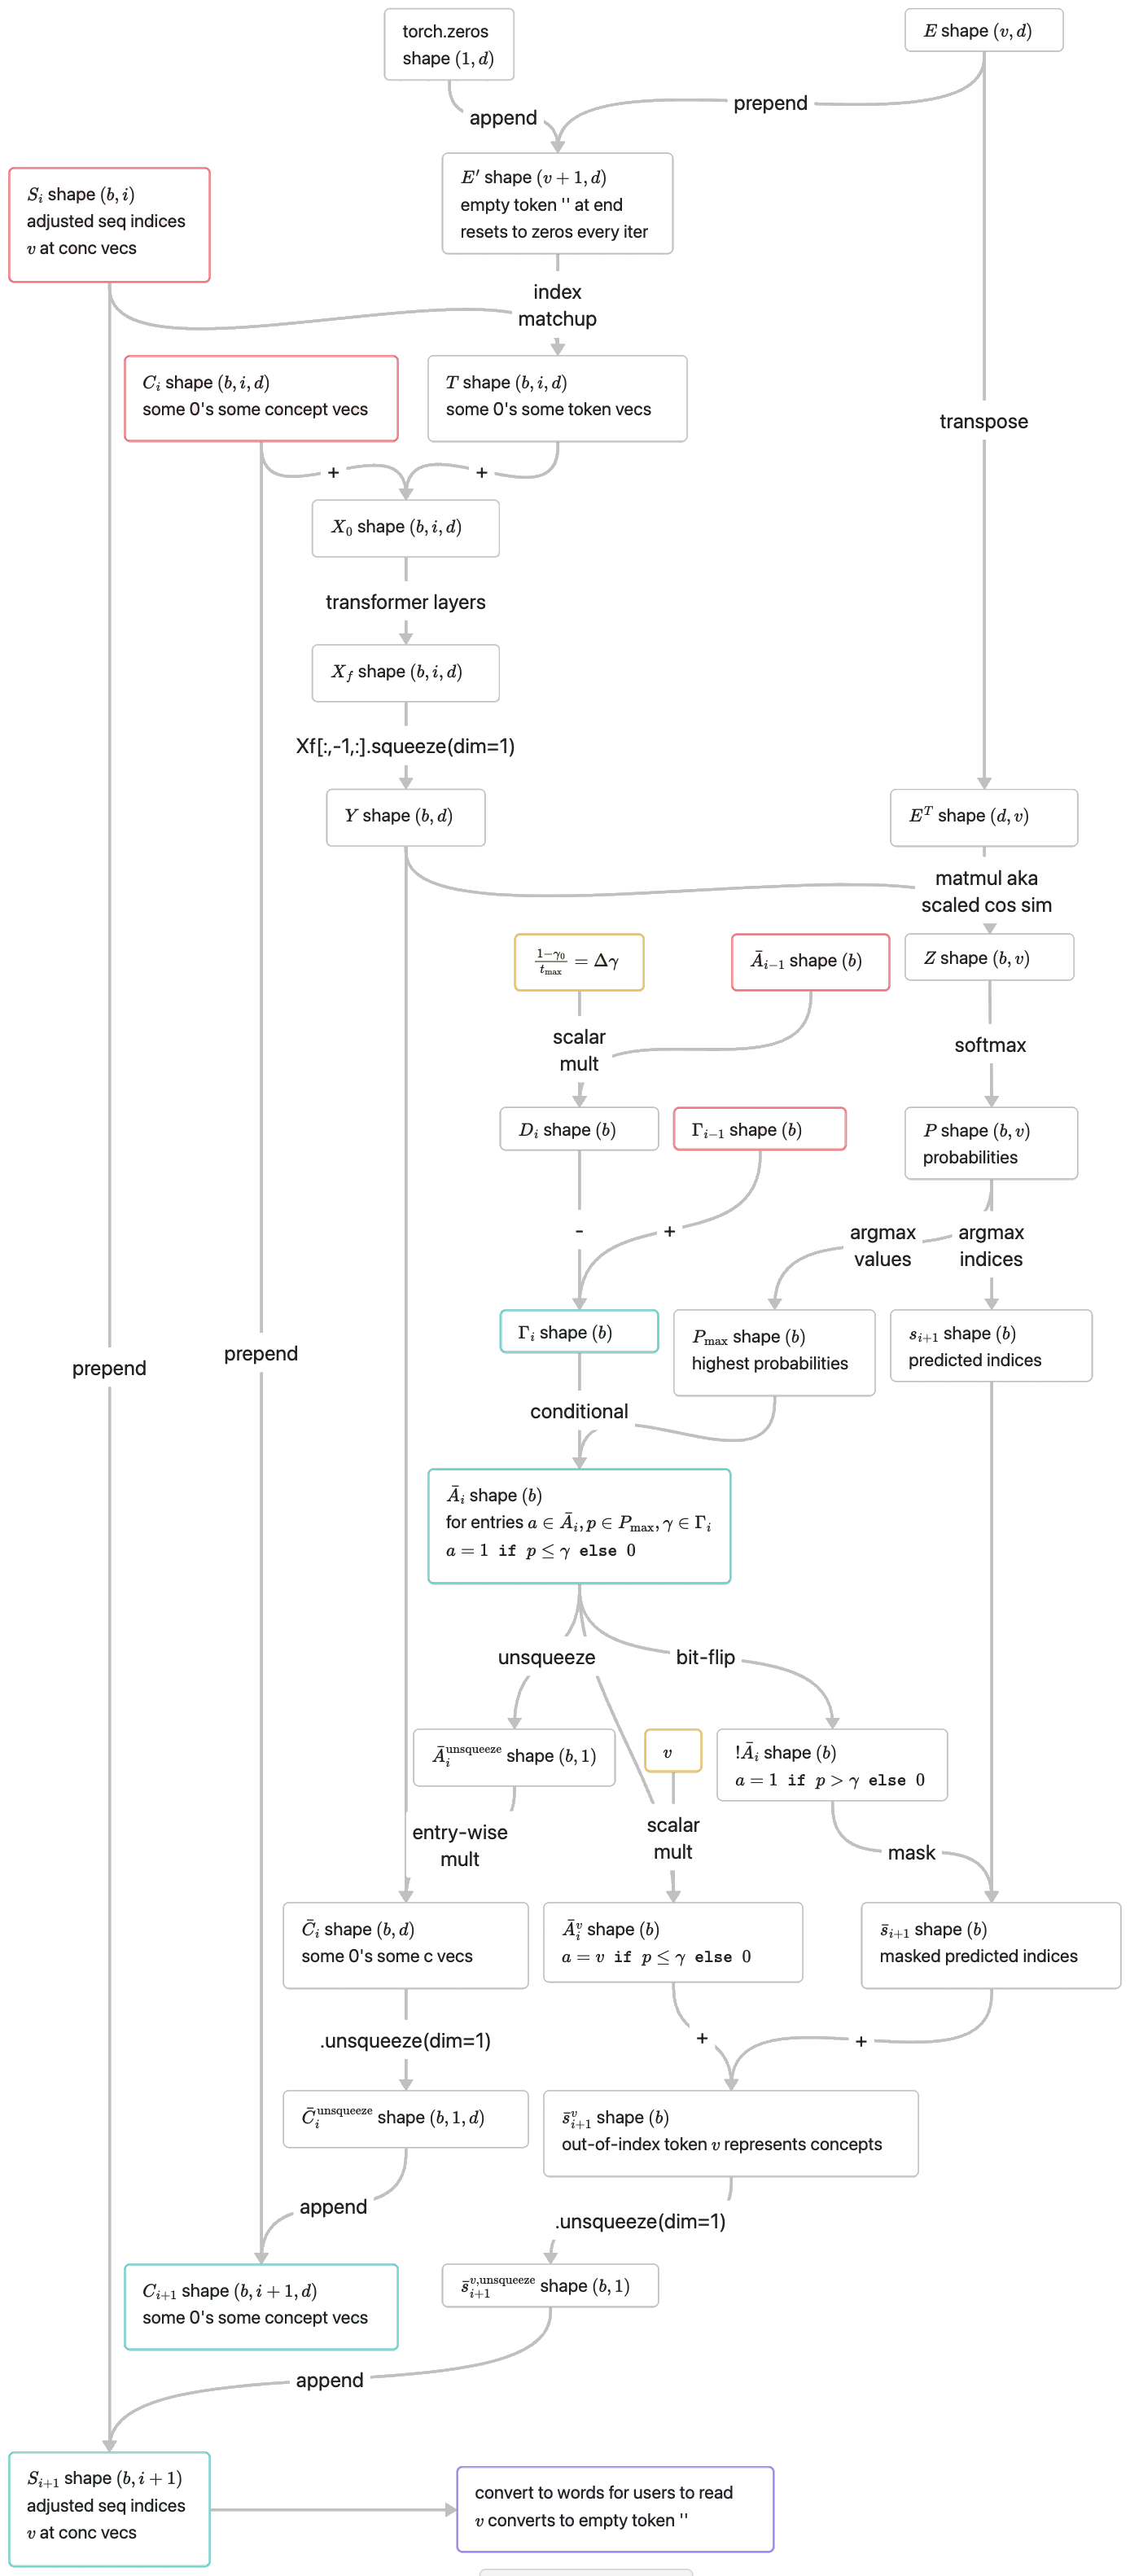
\includegraphics[height=0.9\textheight]{NCP_i>1_inf.png}
    \caption{The way my diagram structure would work for all other steps $(i>1)$ of inference on my next-concept prediction GPT. A yellow box refers to a hyperparameter, red means the object comes from the previous run or from context or the training set, purple means outputted to the user, blue means the object gets sent to be used during the next run, and green means used for backpropogation.}
    \label{fig:ncp_i>1_inf}
\end{figure}

\newpage
\begin{figure}[!htb]
    \centering
    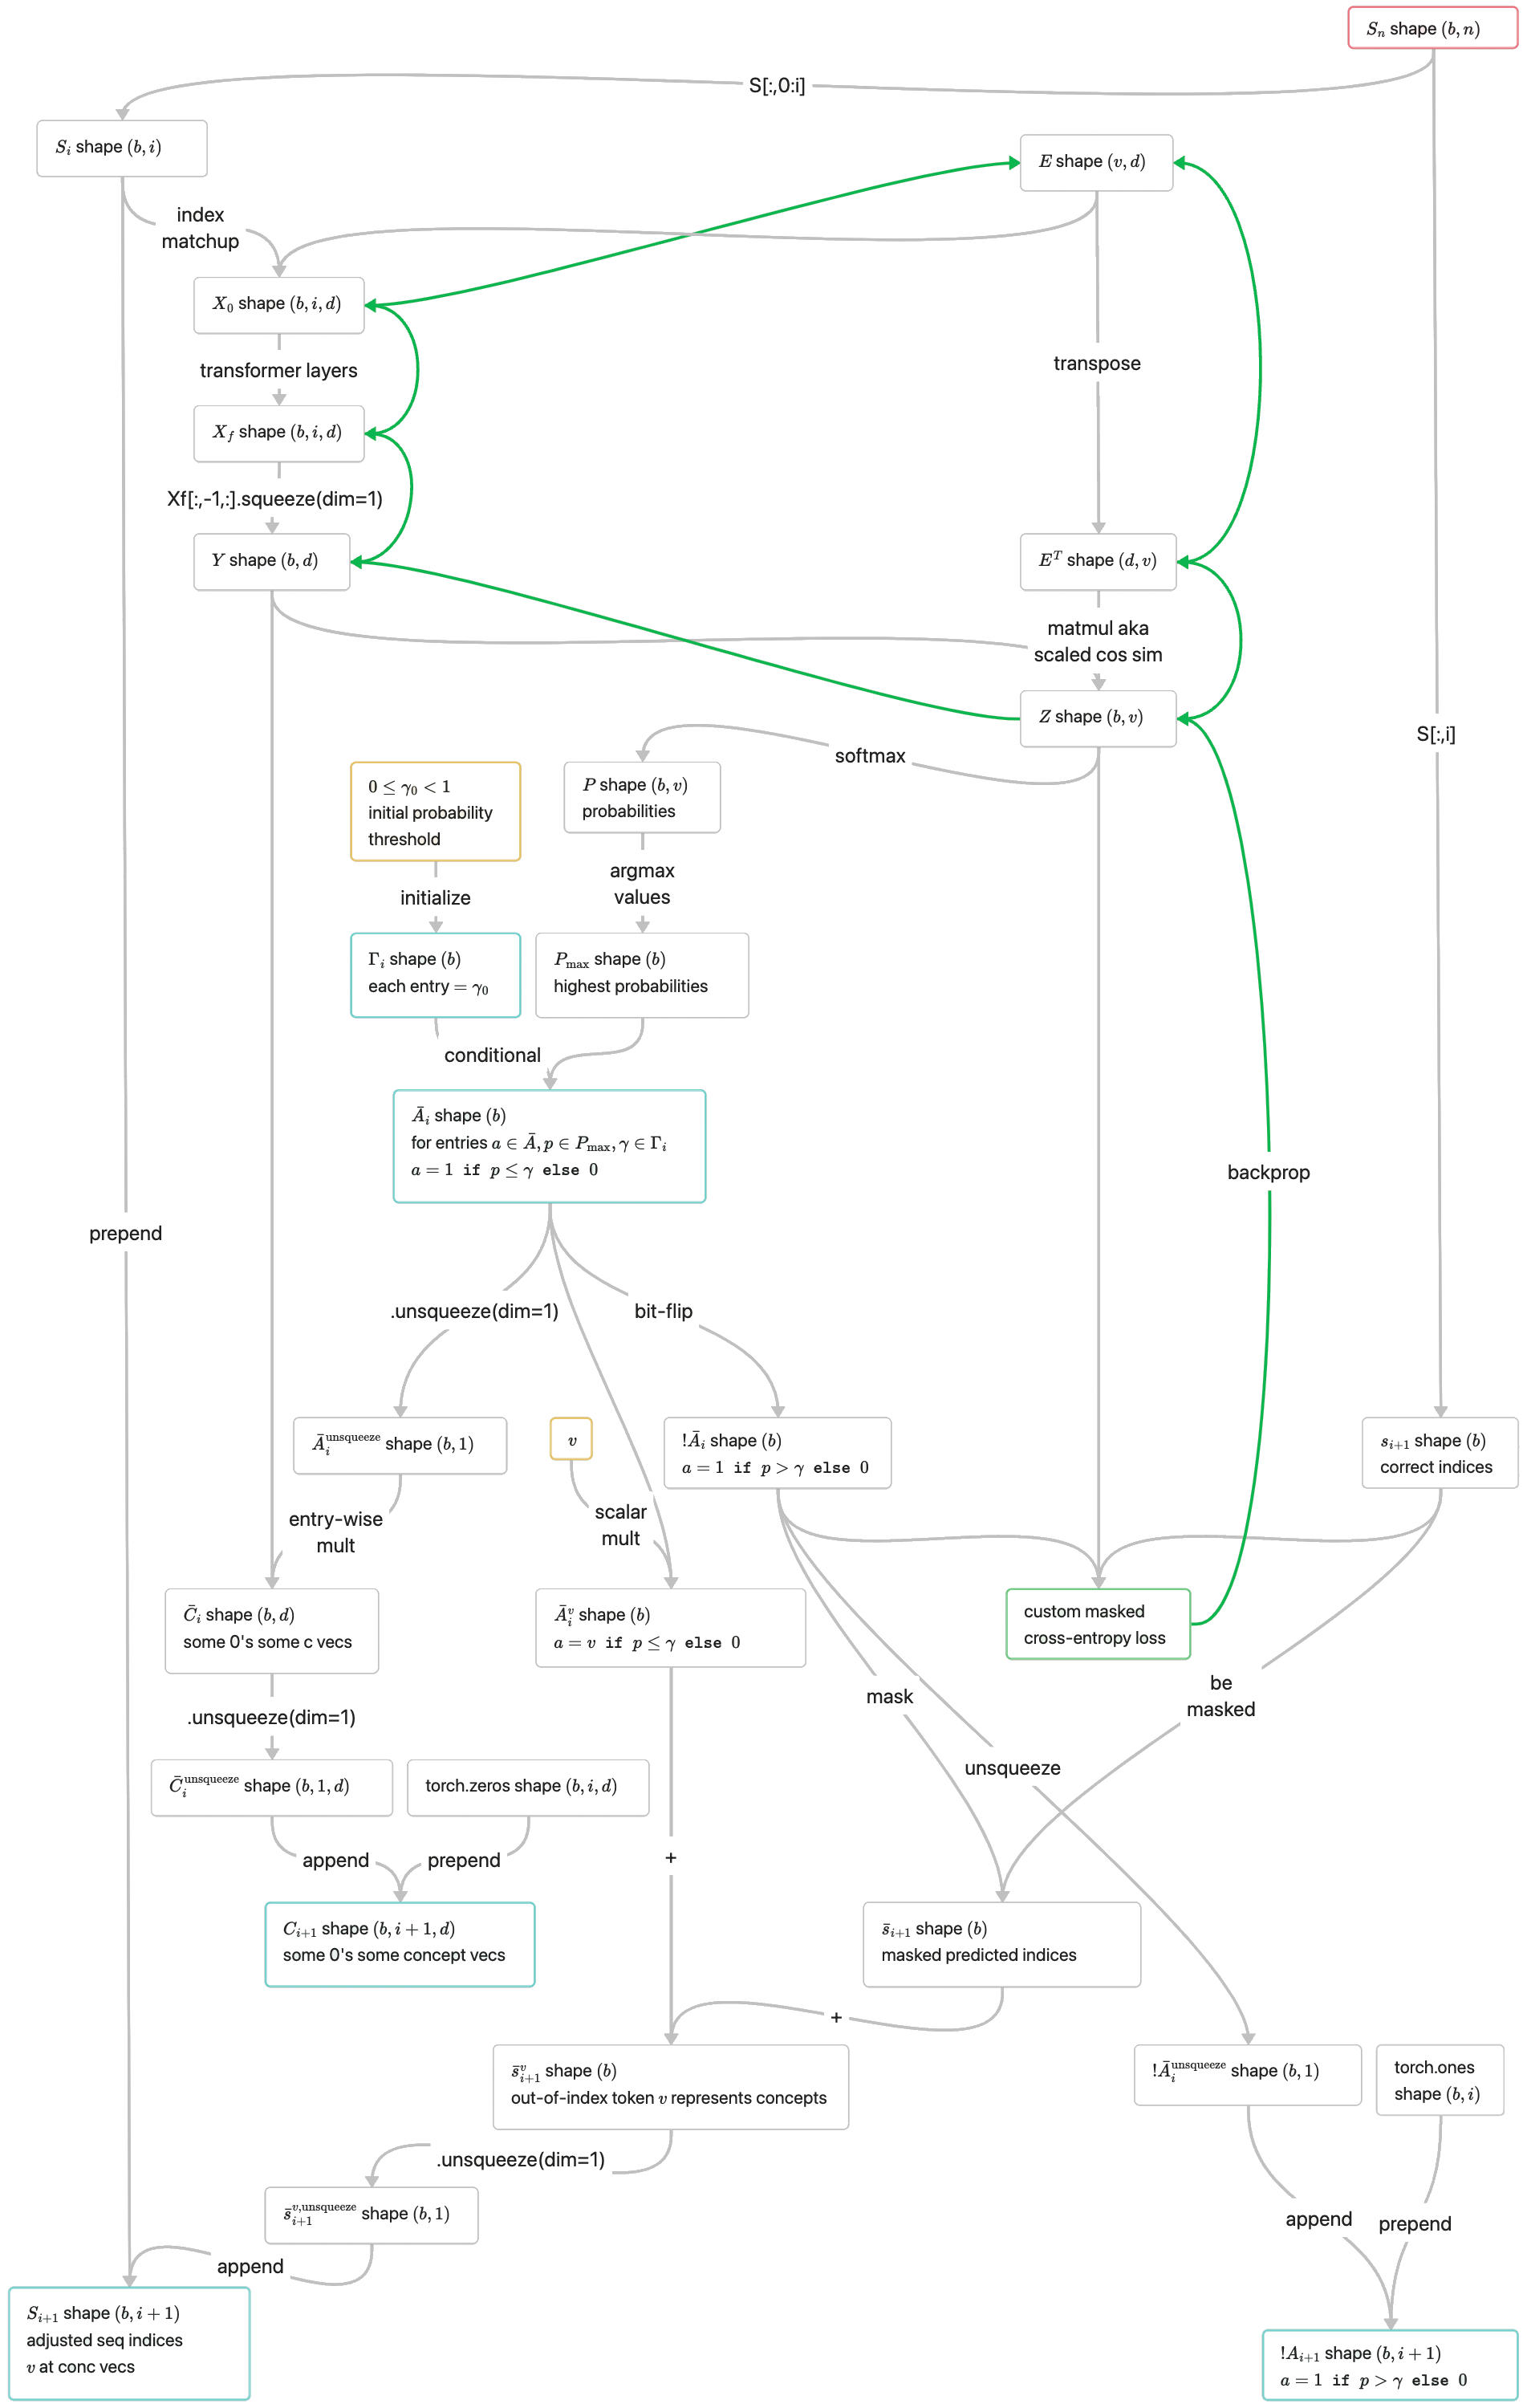
\includegraphics[height=0.9\textheight]{NCP_i=1_train.png}
    \caption{The way my diagram structure would work for the first step $(i=1)$ of training on my next-concept prediction GPT. A yellow box refers to a hyperparameter, red means the object comes from the previous run or from context or the training set, purple means outputted to the user, blue means the object gets sent to be used during the next run, and green means used for backpropogation.}
    \label{fig:ncp_i=1_train}
\end{figure}

\newpage
\begin{figure}[!htb]
    \centering
    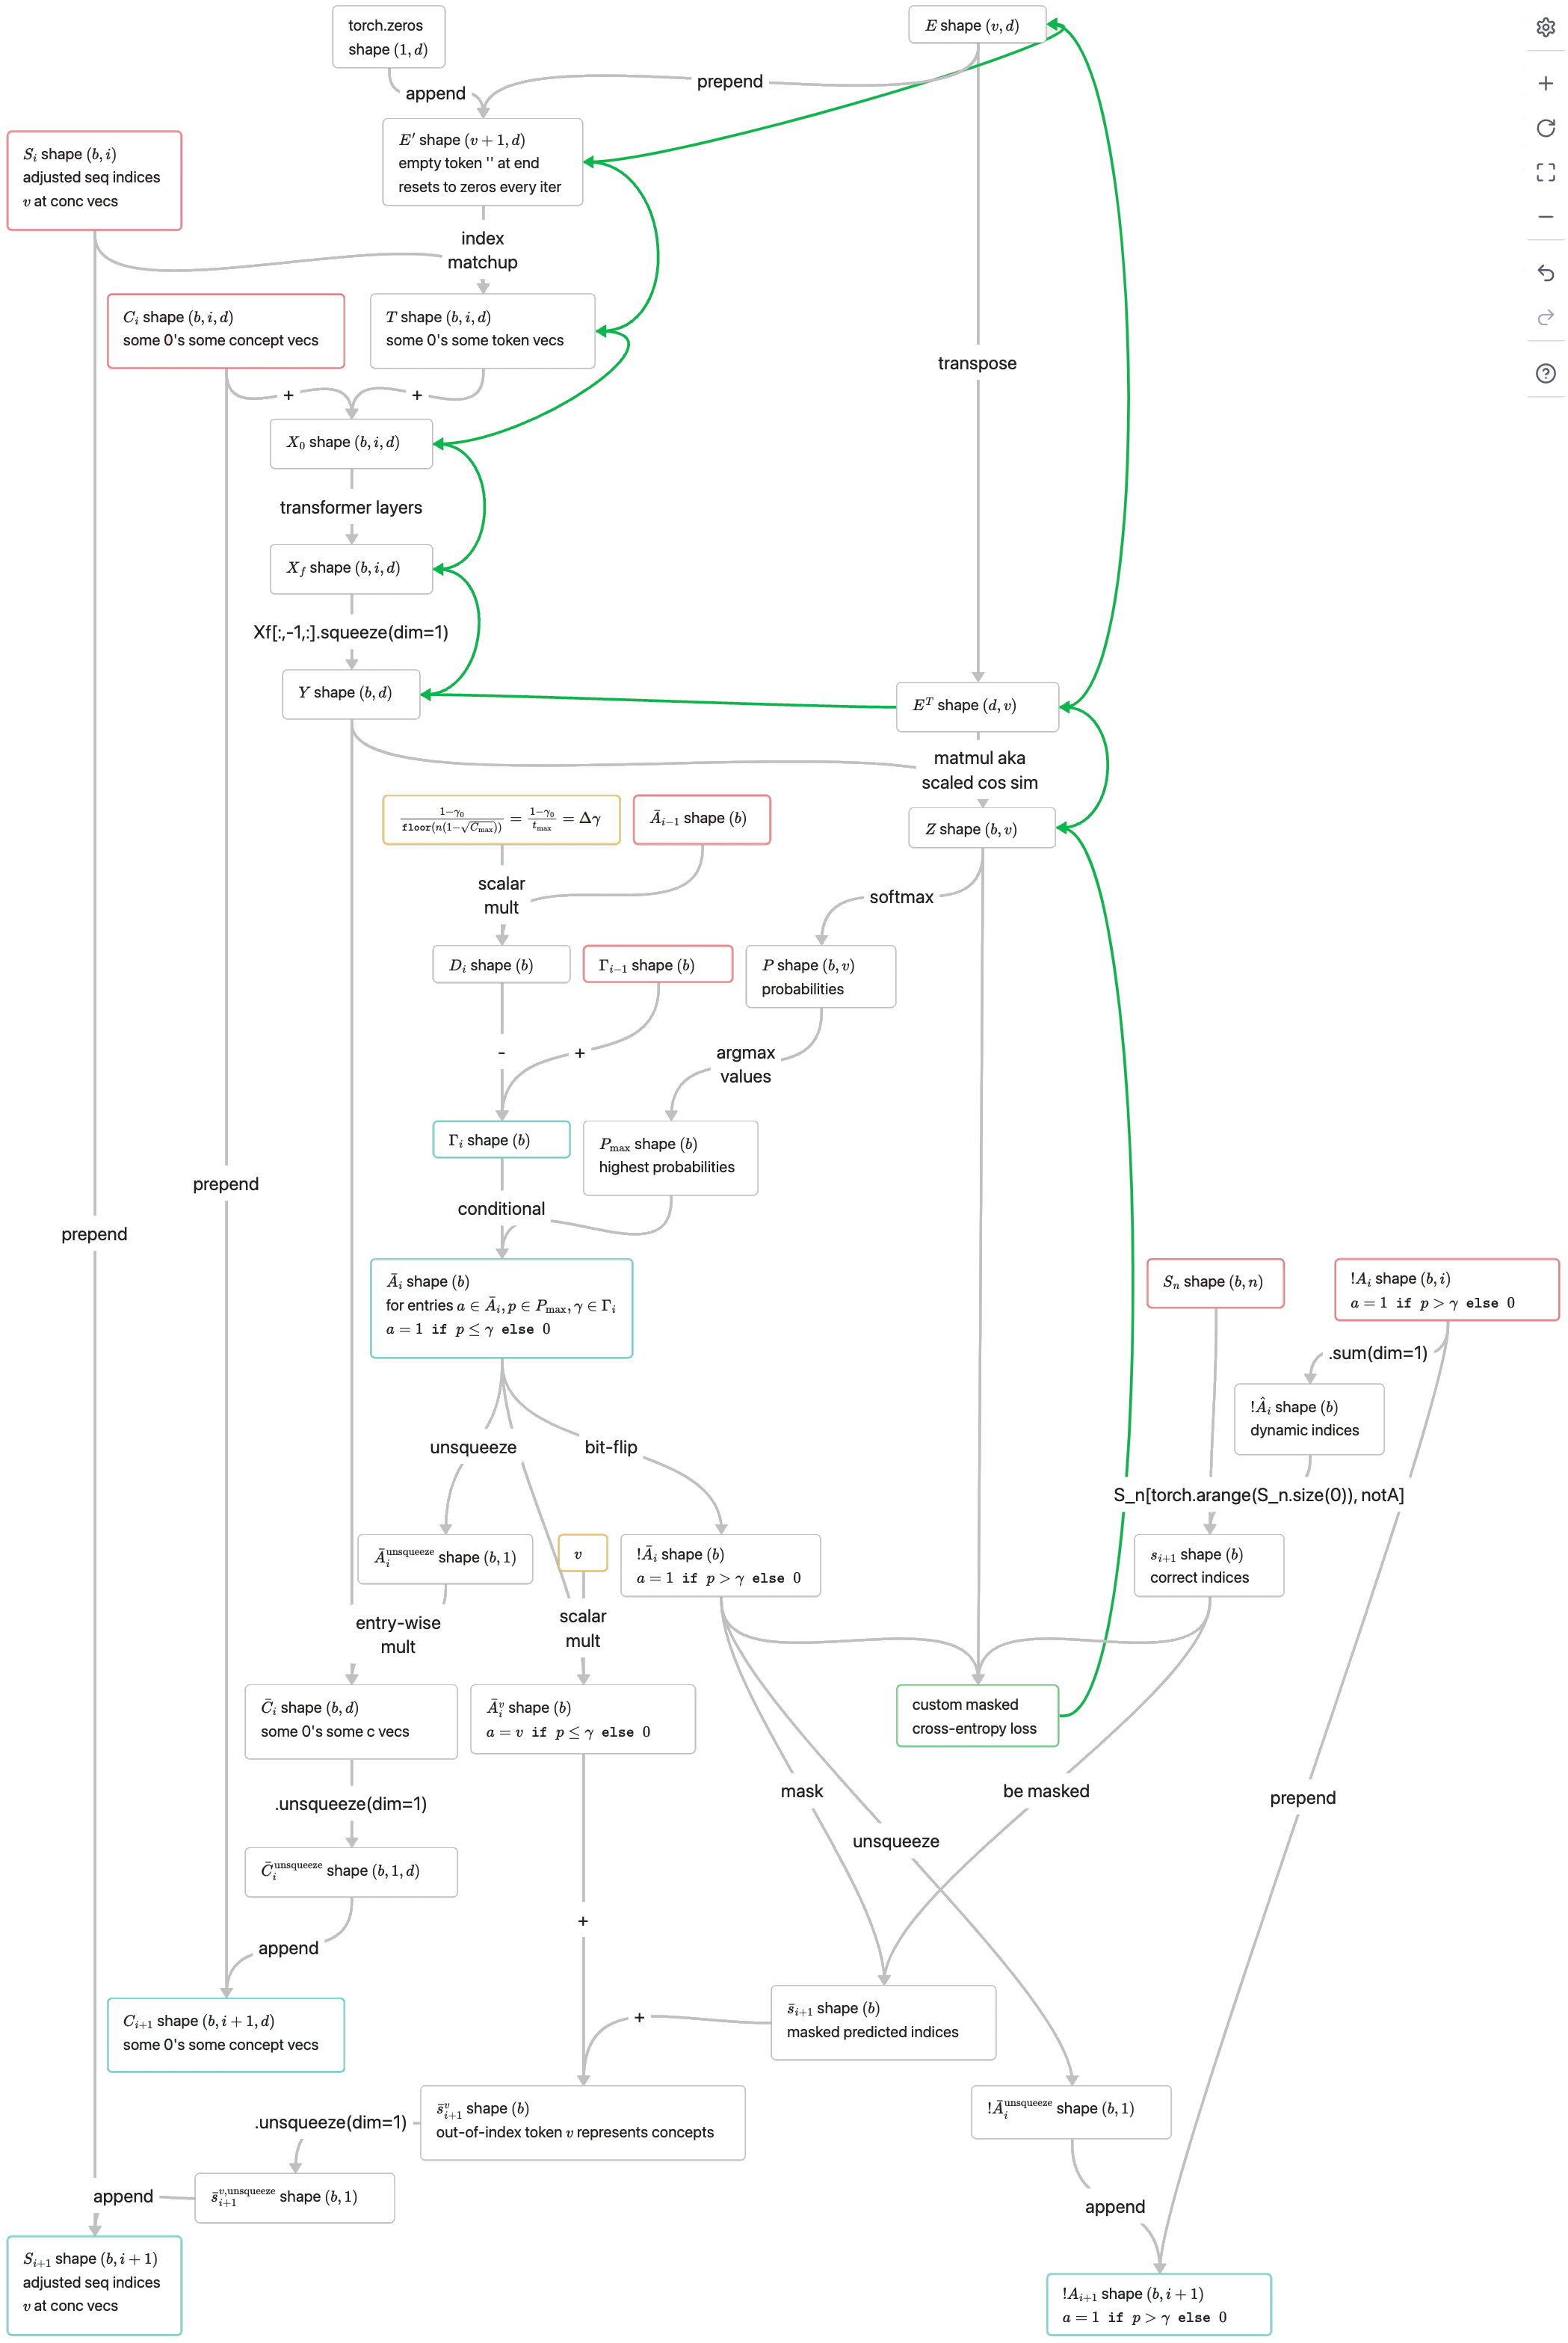
\includegraphics[height=0.9\textheight]{NCP_i>1_train.png}
    \caption{The way my diagram structure would work for all other steps $(i>1)$ of training on my next-concept prediction GPT. A yellow box refers to a hyperparameter, red means the object comes from the previous run or from context or the training set, purple means outputted to the user, blue means the object gets sent to be used during the next run, and green means used for backpropogation.}
    \label{fig:ncp_i>1_train}
\end{figure}



\newpage
\section{Example Algorithm Walkthroug}
\label{sec:example}
For our example walkthrough we'll use a batch size of $b=2$ with the two sequences
$$\begin{matrix}
    \text{" I think therefore I am<endoftext>"} \\
    \text{"Every cloud has a silver lining<endoftext>"}
\end{matrix}$$
which simplifiy into the following tokens
$$S = 
[[\text{" I", " think", " there", "fore", " I", "am", "<endoftext>"}],
[\text{"Every", " cloud", " has", " a", " silver", " lining", "<endoftext>"}]]$$
giving us a minimal embedding matrix $E$ of
$$\begin{bmatrix}
    t_0 & = & \text{" I"}\\
    t_1 & = & \text{" think"}\\
    t_2 & = & \text{" there"}\\
    t_3 & = & \text{" fore"}\\
    t_4 & = & \text{" am"}\\
    t_5 & = & \text{"Every"}\\
    t_6 & = & \text{" cloud"}\\
    t_7 & = & \text{" has"}\\
    t_8 & = & \text{" a"}\\
    t_9 & = & \text{" silver"}\\
    t_{10} & = & \text{" lining"}\\
    t_{11} & = & \text{"<endoftext>"}\\
\end{bmatrix}$$
with $v=12$ and $d=3$.\par

This example will be unrealistic with how often concept vectors are triggered given that relatively small LLMs could finish these sequences with very high confidence.
In reality confidence vectors are more likely to be used in low-certainty scenarios such as math, and we can tune the $\gamma$ value to find a good medium between extra computation and extra performance.

\subsection{Training}



\subsection{Single Sequence Inference}

Here we'll look at just the first sequence.
Notice how the sequence length is $n=7$ which would have us performing inference 6 times in a regular next-token predictor, but here in figure \ref{tab:inf} we end up performing inference 8 times.
This is indeed an increase in computation both in terms of the number of times the model is run and in terms of the $O(n^2)$ complexity of the increased context length in post-concept vector runs.
My hope is that these more recent attempts at linear attention like Mamba work out because my algorithm is orthogonal to them.
If we end up sticking with regular QKV attention tho then my hope is that the increase in training \& inference computation that my model/algorithm creates will be offset by increases in performance. 
Also, remember we set hyperparameter $t_\text{max}$ to limit the maximum additional compute during inference (during training we set $C_\text{max}$ which we use to derive $t_\text{max}$). \par

\begin{figure}[!htb]
    \centering
    \begin{tabular}{|c|c|c|c|c|c|c|}
    i & $\gamma_i$ & input sequence & $X_0$ shape & $p$ & predicted output & $\gamma_{i+1}$\\
    \hline
    1 & 0.5 & " I" & $(1,1,3)$ & 0.52 & " think" & 0.5\\
    2 & 0.5 & " I think" & $(1,2,3)$ & 0.69 & " there" & 0.5\\
    3 & 0.5 & " I think there" & $(1,3,3)$ & 0.43 & $c$ & 0.25\\
    4 & 0.25 & " I think therefore" & $(1,4,3)$ & 0.57 & "fore" & 0.25\\
    5 & 0.25 & " I think therefore" & $(1,5,3)$ & 0.33 & " I" & 0.25\\
    6 & 0.25 & " I think therefore I" & $(1,6,3)$ & 0.21 & $c$ & 0.0\\
    7 & 0.0 & " I think therefore I" & $(1,7,3)$ & 0.44 & " am" & 0.0\\
    8 & 0.0 & " I think therefore I am" & $(1,8,3)$ & 0.87 & "<endoftext>" & \\
\end{tabular}
    \caption{A step-by-step walkthrough of the inference process}
    \label{tab:inf}
\end{figure}

Now let's take a look at table \ref{tab:inf} to get an idea of what's happening during inference in the single sequence case.
It starts off pretty predictable with the first three steps just predicting the next token.
However, at step 4 the output of the model did not meet the criteria of the probability of that token being $>\gamma$, so instead a concept embedding vector was outputted. 
In a normal next-token prediction GPT model, $X_0$ is always created from an index selection between the sequence and embedding dimension.
However, in ours, the model occasionally outputs concept embedding vectors to be appended to $X_0$ and used in the next iteration. 
This makes the loop structure annoying to program ngl.\par

Notice also the columns for $\gamma$.
Assume we set $\gamma=0.5$ as our initial value, meaning a probability of a token coming out of the model's softmax must be at least 50\% or higher in order for it to be classified a token, and otherwise it'll be classified as a concept embedding vector.
Every time a token is outputted, $\gamma$ does not change. 
However, when a concept vector is outputted, $\gamma$ goes down. 
In this specific example I've assumed $\Delta \gamma=0.25$.
$\Delta\gamma$ is defined according to $t_\text{max}$ by $\Delta\gamma = \frac{1-\gamma}{t_\text{max}}$ where $n$ is the sequence length and 1 was chosen to ensure that the final value of $\gamma$ is equivalent to next-token prediction, AKA always choosing to output a token vector.
Here $t_\text{max}$ has been chosen to be 2.
When we do training later, $t_\text{max}$ will be derived from $C_\text{max}$, our maximum allowable compute.


\subsection{Parallel Inference/Training}

I assume showing parallel inference is enough for you to figure out how parallel training works so here's how it looks. Notice how when one sequence is finished it doesn't really matter what it outputs bc we've already hit <endoftext> and have no reason to show anything after that to the user. Here $t_\text{max}$ has been calculated to be 5, thus giving us $\Delta\gamma = 0.1$.
Notice how $\gamma$ changes independently for each sequence and neither sequence happens to reach $\gamma_i=0$ in this example. Also notice that values for $\gamma$ are kept track of individually according to sequence.\par

\begin{figure}[!htb]
    \centering
    \begin{tabular}{|c|c|c|c|c|c|c|}
    i & $(\gamma_i^1,\gamma_i^2)$ & $X_0$ & input sequences & $p$ & outputs & $(\gamma_{i+1}^1,\gamma_{i+1}^2)$ \\
    \hline
    \hline
    1 & $(0.5,0.5)$ & $(2,1,3)$ & " I" & $(0.82,0.31)$ & " think" & $(0.5,0.4)$ \\
    &&& "Every"  && $c$ &\\
    \hline
    2 & $(0.5,0.4)$  & $(2,2,3)$ & " I think" & $(0.54,0.48)$ & " there" & $(0.5,0.4)$ \\
    &&& "Every" && " cloud" &\\
    \hline
    3 & $(0.5,0.4)$  & $(2,3,3)$ & " I think there" & $(0.61,0.38)$ & "fore" & $(0.5,0.3)$ \\
    &&& "Every cloud" && $c$ &\\
    \hline
    4 & $(0.5,0.3)$  & $(2,4,3)$ & " I think therefore" & $(0.21,0.24)$ & $c$ & $(0.4,0.2)$ \\
    &&& "Every cloud" && $c$ &\\
    \hline
    5 & $(0.4,0.2)$  & $(2,5,3)$ & " I think therefore" & $(0.55,0.45)$ & " I" & $(0.4,0.2)$ \\
    &&& "Every cloud" && " has" &\\
    \hline
    6 & $(0.4,0.2)$  & $(2,6,3)$ & " I think therefore I" & $(0.45,0.72)$ & " am" & $(0.4,0.2)$ \\
    &&& "Every cloud has" && " a" &\\
    \hline
    7 & $(0.4,0.2)$  & $(2,7,3)$ & " I think therefore I am" & $(0.35,0.18)$ & $c$ & $(0.3,0.1)$ \\
    &&& "Every cloud has a" && $c$ &\\
    \hline
    8 & $(0.3,0.1)$  & $(2,8,3)$ & " I think therefore I am" & $(0.43,0.66)$ & "<endoftext>" & $(0.3,0.1)$ \\
    &&& "Every cloud has a" && " silver" &\\
    \hline
    9 & $(0.3,0.1)$  & $(2,9,3)$ & " I think therefore I am<endoftext>" & $(\_,0.63)$ &  & $(0.3,0.1)$ \\
    &&& "Every cloud has a silver" && " lining" &\\
    \hline
    10 & $(0.3,0.1)$  & $(2,10,3)$ & " I think therefore I am<endoftext>" & $(\_,0.44)$ &  & \\
    &&& "Every cloud has a silver lining" && "<endoftext>" &\\
    \end{tabular}
    \caption{Parallel inference / batched training}
    \label{fig:enter-label}
\end{figure}


\newpage
\section{Conclusion}
Your conclusion here

\section*{Acknowledgments}
This was was supported in part by......

%Bibliography
\bibliographystyle{unsrt}  
\bibliography{references}  


\end{document}
